% !TEX TS-program = xelatex
% !TEX encoding = UTF-8 Unicode
% !Mode:: "TeX:UTF-8"

\documentclass{resume}
\usepackage{multirow}
\usepackage{zh_CN-Adobefonts_external} % Simplified Chinese Support using external fonts (./fonts/zh_CN-Adobe/)
% \usepackage{NotoSansSC_external}
% \usepackage{NotoSerifCJKsc_external}
% \usepackage{zh_CN-Adobefonts_internal} % Simplified Chinese Support using system fonts
\usepackage{linespacing_fix} % disable extra space before next section
\usepackage{cite}

\begin{document}
\pagenumbering{gobble} % suppress displaying page number
\name{王康宁}
\basicInfo{
  \email{corningwkn@163.com} \textperiodcentered\ 
  \phone{(+86) 180-5510-5668} \textperiodcentered}
  %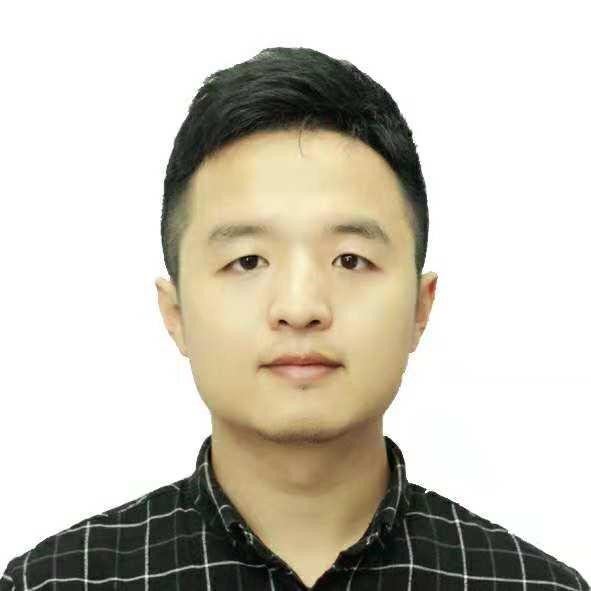
\includegraphics[width=0.88in]{avatar}}
\section{\faGraduationCap\  教育背景}
\datedsubsection{\textbf{西安电子科技大学}, 西安, 陕西}{2008 -- 2012}
信息工程\textit{学士}

\section{\faUsers\  工作经历}
\datedsubsection{\textbf{奇瑞汽车股份有限公司}	芜湖}{2019年10月至今}
\role {主管工程师}

奇瑞汽车售前DMS、奇瑞新能源售前DCS项目的二次设计和开发
\begin{onehalfspacing}
\begin{itemize}
  \item 负责基于ABP框架和RESTful风格的.net core后端项目二次开发
  \item 负责搭建基于k8s,docker和gitlab的持续集成和自动部署
  \item 负责管理小组成员日常开发工作及review后端代码
\end{itemize}
\end{onehalfspacing}

\datedsubsection{\textbf{浙江网新恒天软件有限公司}	合肥}{2015年6月 -- 2019年9月}
\role{高级工程师}

Jeppesen公司为波音公司提供的地图打印服务
\begin{onehalfspacing}
\begin{itemize}
  \item 带领项目组到国外现场和客户对接需求以及安排日常的开发工作
  \item 使用Redis存储定时任务和缓存结果,使用kafka做消息队列服务,处理大量业务数据
  \item 负责基于asp.net core mvc + vue全家桶的项目开发和sql server数据库设计
\end{itemize}
\end{onehalfspacing}

\datedsubsection{\textbf{安徽科力信息产业有限公司}	合肥}{2012 年7月 -- 2015年3月}
\role{.net开发工程师}

安徽高速交警监控系统、管控平台等
\begin{onehalfspacing}
\begin{itemize}
  \item 基于winform和ado.net的视频监控及定位软件
  \item 开发基于gis地图的相关winform控件
  \item 优化视频流媒体数据的处理,包括录像、存储、查看等功能
\end{itemize}
\end{onehalfspacing}

\section{\faCogs\ 工作技能}
% increase linespacing [parsep=0.5ex]
\begin{itemize}[parsep=0.5ex]
  \item 编程语言: c\#, sql, html, javascript
  \item 框架: .net core,EF Dapper等ORM框架
  \item 数据库: sqlserver, oracle, redis
  \item 设计: UML, office系列
  \item 其他: git及工具, jenkins, RESTful, 常用设计模式
  \item 语言: 英语cet-6, 听说读写熟练
\end{itemize}

\section{\faInfo\ 其他}
% increase linespacing [parsep=0.5ex]
\begin{itemize}[parsep=0.5ex]
  \item 技术博客: http://cnblogs.com/corning91
  \item GitHub: https://github.com/Corning91
\end{itemize}

%% Reference
%\newpage
%\bibliographystyle{IEEETran}
%\bibliography{mycite}
\end{document}
